\input ../SlidePreamble
\input ../preamble

\newcommand{\solution}[1]{\bigskip {\bf Solution}: #1}

\begin{document}

{\Huge
  \centerline{\bf TTIC 31230, Fundamentals of Deep Learning}
  \bigskip
  \centerline{David McAllester, Winter 2018}
  \vfill
  \centerline{\bf Stochastic Gradient Descent (SGD)}
  \vfill
  \centerline{The Classical Convergence Thoerem}
  \vfill
  \centerline{RMSProp, Momentum and Adam}
  \vfill
  \centerline{Scaling Learning Rates with Batch Size}
  \vfill
  \centerline{Gradient Flow and Langevin Dynamics}
  
\slide{Vanilla SGD}

$$\Phi \;\minuseq\; \eta \hat{g}$$

\vfill
\begin{eqnarray*}
  \hat{g} & = & E_{(x,y) \sim \mathrm{Batch}}\;\nabla_\Phi\;\mathrm{loss}(\Phi,x,y) \\
  \\
  \\
  g & = & E_{(x,y) \sim \mathrm{Pop}}\;\nabla_\Phi\;\mathrm{loss}(\Phi,x,y) \\
\end{eqnarray*}

\slide{Issues}

\vfill
\begin{itemize}
\item {\bf Gradient Estimation.} The accuracy of $\hat{g}$ as an estimate of $g$.

  \vfill
\item {\bf Gradient Drift (second order structure).} The fact that $g$ changes as the parameters change.

  \vfill
\item {\bf Convergence.} To converge to a local optimum the learning rate must be gradually reduced toward zero.

  \vfill
  \item {\bf Exploration.} Since deep models are non-convex we need to search over the parameter space.  SGD can behave like MCMC.
\end{itemize}

\slide{A One Dimensional Example}

Suppose that $y$ is a scalar, and consider

\begin{eqnarray*}
 \mathrm{loss}(\beta,y) & = & \frac{1}{2}(\beta - y)^2 \\
 \\
  g & = & E_{y \sim \mathrm{Pop}}\; \nabla_\beta\;\frac{1}{2}(\beta - y)^2 \\
  \\
  & = & \beta - E_{y \sim \mathrm{Pop}} \; y \\
  \\
  \hat{g} & = &\beta - E_{y \sim \mathrm{Batch}} \;y
\end{eqnarray*}

\vfill
Even if $\beta$ is optimal, for a finite batch we will have $\hat{g} \not = 0$.

\slide{The Classical Convergence Theorem}

$$\Phi \;\minuseq \; \eta_t \nabla_\Phi\;\mathrm{loss}(\Phi,x_t,y_t)$$

\vfill
For ``sufficiently smooth'' non-negative loss with

\vfill
$$\eta_t > 0\;\;\;\;\mbox{and}\;\;\;\;\lim_{t \rightarrow 0} \;\eta_t = 0\;\;\;\;\mbox{and}\;\;\;\;\sum_t \eta_t = \infty,$$

\vfill
we have that the training loss of $\Phi$ converges (in practice $\Phi$ converges to a local optimum of training loss).

\vfill
{\Large {\bf Rigor Police:} One can construct cases where $\Phi$ converges to a saddle point or even a limit cycle.}

\vfill
{\Large See ``Neuro-Dynamic Programming'' by Bertsekas and Tsitsiklis proposition 3.5.}

\slide{Physicist's Proof of the Convergence Theorem}

Since $\lim_{t \rightarrow 0} \;\eta_t = 0$ we will eventually get to arbitrarilly small learning rates.

\vfill
For sufficiently small learning rates any meaningful update of the parameters will be based on an arbitrarily large sample
of gradients at essentially the same parameter value.

\vfill
An arbitrarily large sample will become arbitrarily accurate as an estimate of the full gradient.

\vfill
But since $\sum_t \eta_t = \infty$, no matter how small the learning rate gets, we still can make arbitrarily large motions in parameter space.

\slidetwo{SGD as a form of MCMC}{Learning Rate as a Temperature Parameter}

\centerline{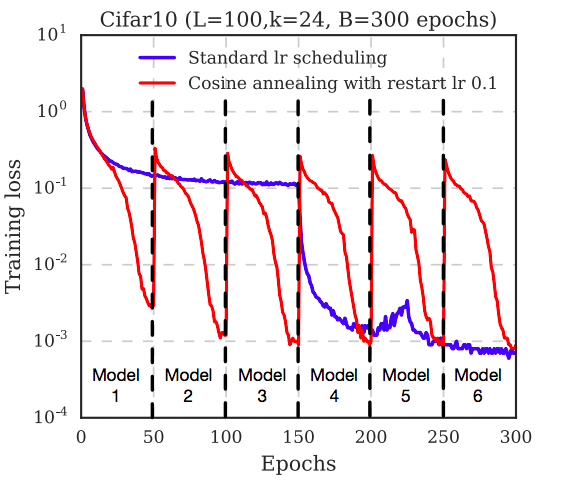
\includegraphics[height= 4in]{../images/AnnealingSGD}}
\centerline{\Large Gao Huang et. al., ICLR 2017}

\slide{}
\centerline{\bf Standard Non-Vanilla SGD Algorithms}
\vfill
\vfill

\slideplain{Digression on Running Averages}
Consider a sequence $x_1$, $x_2$, $x_3$, $\ldots$.
\vfill
For $t \geq N$, consider the average of the $N$ most recent values.
$$\tilde{\mu} = \frac{1}{N} \sum_{s=t-N+1}^t x_s$$

\vfill
This can be approximated more efficiently with
\begin{eqnarray*}
\hat{\mu}_0 & = & 0 \\
\\
\hat{\mu}_t & = & \left(1-\frac{1}{N}\right)\hat{\mu}_{t-1} + \left(\frac{1}{N}\right)x_t\;\;\;t \geq 1 \\
\\
\hat{\mu}_t & \approx & \tilde{\mu}_t \;\;\; t >N
\end{eqnarray*}

\slide{Running Averages}

More explicitly, for $\hat{\mu}_0 = 0$, the update

$$\hat{\mu}_t = \left(1-\frac{1}{N}\right)\hat{\mu}_{t-1} + \left(\frac{1}{N}\right)x_t$$

\vfill
gives

$$\hat{\mu}_t = \frac{1}{N} \sum_{1 \leq s \leq t} \left(1-\frac{1}{N}\right)^{-(t-s)} x_s$$

\vfill
where we have

$$\sum_{n\geq 0} \left(1-\frac{1}{N}\right)^{-n} = N$$

\slide{RMSProp}

RMSProp is based on a running average of $\hat{g}[i]^2$ for each real-valued model parameter $i$.

\begin{eqnarray*}
{\color{red} s_t[i]} & {\color{red} =} & {\color{red} \left(1-\frac{1}{N_s}\right) s_{t-1}[i] + \frac{1}{N_s} \hat{g}_t[i]^2}\;\;\;\mbox{$N_s$ typically 100 or 1000} \\
\\
{\color{red} \Phi_{t+1}[i]} & {\color{red} =} & {\color{red} \Phi_t[i] - \frac{\eta}{\sqrt{s_t[i] + \epsilon}}\;\; \hat{g}_t[i]} \\
\\
\\
s[i] & \approx & E\;\hat{g}[i]^2  =  g[i]^2 + \sigma[i]^2
\end{eqnarray*}

\vfill
We should expect $\sigma[i] >> g[i]$.

\slide{Momentum}

\begin{eqnarray*}
  {\color{red} v_t} & {\color{red} =} & {\color{red} \left(1-\frac{1}{N}\right) v_{t-1} + \eta * \hat{g}_t} \\
  \\
  {\color{red} \Phi_{t+1}} & {\color{red} =} & {\color{red} \Phi_t -  v_t} \\
\end{eqnarray*}

The theory of momentum is generally given in terms of second order structure.


\centerline{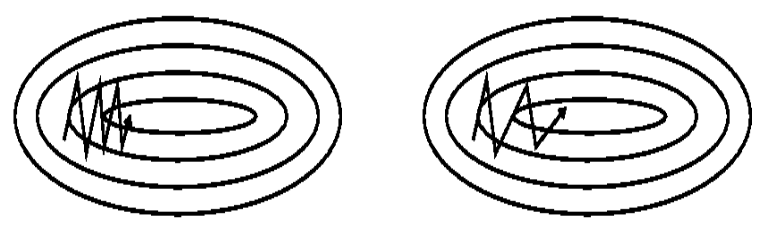
\includegraphics[width = 4in]{../images/momentum}}
\centerline{\Large Rudin's blog}

\slideplain{Momentum}

However, second order analyses are controversial in Deep Learning.

\vfill
We can perhaps get insight by reparameterizing the momentum equations.

\slide{A Reparameterization}

\begin{eqnarray*}
v_t & = & \left(1-\frac{1}{N}\right) v_{t-1} + \eta \hat{g}_t \\
\\
& = & \left(1-\frac{1}{N}\right) v_{t-1} + \frac{1}{N}(N\eta \hat{g}_t) \\
\\
& = & N\eta\mu_t\;\;\mbox{for}\;{\color{red} \mu_t = \left(1-\frac{1}{N}\right)\mu_{t-1} + \frac{1}{N} \hat{g}_t} \\
\\
\Phi_{t+1} & = & \Phi_t - v_t \\
\\
& = & \Phi_t - {\color{red} N\eta\mu_t} 
\end{eqnarray*}

\slide{A Reparameterization}

\begin{eqnarray}
{\color{red} \mu_t} & {\color{red} =} & {\color{red} \left(1-\frac{1}{N_{\mu}}\right)\mu_{t-1} + \frac{1}{N_{\mu}} \hat{g}_t}\;\;N_{\mu}\;\mbox{typically 10 or 100} \nonumber \\
\nonumber \\
\label{eq:momentum1}
\Phi_{t+1} & = & \Phi_t - N\eta\mu_t \\
\nonumber\\
 \label{eq:momentum2}
 & = & {\color{red} \Phi_t - \eta'\mu_t}
\end{eqnarray}

My intuition: For the parameterization $N$ and $\eta'$ defined by (\ref{eq:momentum2}) it should be possible to optimize $N$ and $\eta'$ largely independently.
I would not expect this to be true for the $N$ and $\eta$ defined by (\ref{eq:momentum1}).

\slide{Adam --- Adaptive Momentum}

Adam combines momentum and RMSProp.

\vfill
It also uses ``bias correction'' of running averages.

\slide{A Digression on Bias Correction of Running Averages}

Consider a sequence $x_1,\;x_2,\;x_3,\ldots$ and consider the following for $N$ large.

\begin{eqnarray*}
\hat{\mu}_0 & = & 0 \\
\\
\hat{\mu}_t & = & \left(1-\frac{1}{N}\right)\hat{\mu}_{t-1} + \left(\frac{1}{N}\right)x_t
\end{eqnarray*}

\vfill
For $\mu \doteq E\;x$ we have $E\;\hat{\mu}_1 = \mu/N$.

\vfill
For $t << N$ we have $E\;\hat{\mu}_t \approx (t/N)\mu$.

\slide{Bias Correction of Running Averages}

The following running average maintains the invariant that $\hat{\mu}_t$ is exactly the average of $x_1,\ldots,x_t$.

\begin{eqnarray*}
\hat{\mu}_0 & = & 0 \\
\\
\hat{\mu}_t & = & \left(1-\frac{1}{t}\right)\hat{\mu}_{t-1} + \left(\frac{1}{t}\right)x_t
\end{eqnarray*}

\vfill
But this fails to track a moving average for $t >> N$.

\slide{Bias Correction of Running Averages}

The following avoids the initial bias toward zero while still tracking a moving average.

\begin{eqnarray*}
\hat{\mu}_0 & = & 0 \\
\\
\hat{\mu}_t & = & \left(1-\frac{1}{\min(N,t)}\right)\hat{\mu}_{t-1} + \left(\frac{1}{\min(N,t)}\right)x_t
\end{eqnarray*}

\vfill
The published version of Adam has a more obscure form of bias correction which yields essentially the same effect.

\slide{Adam (simplified)}

\begin{eqnarray*}
  \mu_0[i] & = & s_0[i] = 0 \\
  \\
  \mu_{t}[i] & = & \left(1-\frac{1}{\min(t,N_g)}\right)\mu_{t-1}[i] + \frac{1}{\min(t,N_g)} \hat{g}_t[i] \\
  \\
  s_{t}[i] & = & \left(1-\frac{1}{\min(t,N_s)}\right)s_{t-1}[i] + \frac{1}{\min(t,N_s)} \hat{g}_t[i]^2 \\
  \\
\Phi_{t+1}[i] & =  & \Phi_t - \frac{\eta}{\sqrt{s_{t}[i] + \epsilon}}\;\;\mu_{t}[i]
\end{eqnarray*}

\slide{Scaling $\eta$, $N_{\mu}$ and $N_s$ with Batch Size}

Recent work has show that scaling hyper-parameters with the batch size can lead to effective learning with very large (highly parallel)
batches.

\vfill
{\bf Accurate, Large Minibatch SGD: Training ImageNet in 1 Hour}, Goyal et al., 2017.

\vfill
{\bf Don't Decay the Learning Rate, Increase the Batch Size}, Smith et al., 2018

\slide{Scaling $\eta$}

Consider two consecutive updates for a batch size of 1 with learning rate $\eta_1$.

\begin{eqnarray*}
  \Phi_{t+1} & = & \Phi_t - \eta_1 \nabla_\Phi \mathrm{loss}(\Phi_t,x_t,y_t) \\
  \\
  \Phi_{t+2} & = & \Phi_{t+1} - \eta_1 \nabla_\Phi \mathrm{loss}(\Phi_{t+1},x_{t+1},y_{t+1}) \\\
  \\
  & \approx & \Phi_{t+1} - \eta_1 \nabla_\Phi \mathrm{loss}(\Phi_t,x_{t+1},y_{t+1}) \\
  \\
  & = & \Phi_t - \eta_1((\nabla_\Phi \mathrm{loss}(\Phi_t,x_t,y_t)) + (\nabla_\Phi \mathrm{loss}(\Phi_t,x_{t+1},y_{t+1})))
\end{eqnarray*}

\slide{Scaling $\eta$}

Let $\eta_B$ be the learning rate for batch size $B$.

\vfill
\begin{eqnarray*}
  \Phi_{t+2} & \approx & \Phi_t - \eta_1((\nabla_\Phi \mathrm{loss}(\Phi_t,x_t,y_t)) + (\nabla_\Phi \mathrm{loss}(\Phi_t,x_{t+1},y_{t+1}))) \\
  \\
  & = & \Phi_t - 2\eta_1\;\hat{g}\;\;\;\mathrm{for}\;\;B=2
\end{eqnarray*}

\vfill
Hence two updates with $B=1$ at learning rate $\eta_1$ is the same as one update at $B=2$ and learning rate $2\eta_1$.

\vfill
$$\eta_2 = 2\eta_1,\;\;\;\;\;\;{\color{red} \eta_B = B\eta_1}$$

\slide{Scaling $N_\mu$}

Let $N_{\mu,B}$ be the momentum parameter to be used with batch size $B$.

\vfill
For batch size $B$, $\hat{\mu}_t$ is averaging over $N_{\mu,B}B$ gradient values.

\vfill
Holding the number of included gradients constant gives

\vfill
$${\color{red} N_{\mu,B}B = N_{\mu,1}\;\;\;\mbox{or}\;\;\;N_{\mu,B} = N_{\mu,1}/B}$$

\slide{Scaling $N_s$}

The simple analysis for $N_{\mu}$ fails for $N_s$.

\vfill
To estimate $E\;g[i]^2$ we should average $\hat{g}_t[i]^2$ over batch elements rather than batch averages.

\vfill
The parameter $N_s$ should be a number of gradients (batch elements) rather than a number of batches,

\vfill Under this semantics, $N_s$ should be constant independent of batch size.

\slide{Gradient Flow}

Consider the differential equation

$${\color{red} \frac{d \Phi}{d t} = - g(\Phi) \;\;\;\;\;\; g(\Phi) = \nabla_\Phi\; E_{(x,y) \sim \mathrm{Train}}\;{\cal L}(\Phi,x,y)}$$

\vfill
Let $\Phi(t)$ be the solution satisfying $\Phi(0) = \Phi_{\mathrm{init}}$.

\vfill
For small values of $\Delta t$ this differential equation can be approximated by

\vfill
$${\color{red} \Delta \Phi = - g(\Phi)\Delta t}$$

\vfill
Here $\Delta t$ can be interpreted as a learning rate.

\slide{Gradient Flow}

$${\color{red} \Delta \Phi = - g(\Phi)\Delta t}$$

\vfill
For a given value of $t$ and $N$ let $\Phi_j$ be defined by

\vfill
\begin{eqnarray*}
\Phi_0 & = & \Phi_{\mathrm{init}} \\
\\
\Phi_{j+1} & = & \Phi_j - \left(\frac{t}{N}\right) g(\Phi_j)
\end{eqnarray*}

\vfill
$${\color{red} \lim_{N\rightarrow \infty} \;\Phi_N = \Phi(t)}$$


\slide{Progress Theorem for Gradient Flow}

\begin{eqnarray*}
  \frac{d \ell}{d t} & = & (\nabla_\Phi \;\ell(\Phi)) \cdot \frac{d \Phi}{dt} \\
  \\
  & = & - (\nabla_\Phi \;\ell(\Phi)) \cdot (\nabla_\Phi \;\ell(\Phi)) \\
  \\
  & = & - ||\nabla_\Phi \;\ell(\Phi)||^2 \\
  \\
  & \leq & 0
\end{eqnarray*}

\vfill
If $\ell(\Phi) \geq 0$ then $\ell(\Phi)$ must converge to a limiting value.

\vfill
This does not imply that $\Phi$ converges.

\slide{SGD also yields Gradient Flow}
For
$$\Phi_{j+1} = \Phi_j - \left(\frac{t}{N}\right) {\color{red} \hat{g}_j}$$
we still have

\vfill
$${\color{red} \lim_{N\rightarrow \infty} \;\Phi_N = \Phi(t)}$$

\vfill
To see this note that we can divide the updates into $\sqrt{N}$ blocks each of size $\sqrt{N}$.  The ``time'' spent within each block is $t/\sqrt{N}$ which converges to 0.
But the number of updates within each block grows as $\sqrt{N}$ and hence the average update within a block converges to $g$.


\slide{Langevin Dynamics}

Consider actual gradient descent
$$\Phi_{j+1} = \Phi_j - \eta\hat{g}_j$$

\vfill
Inspired by gradient flow, we define time by $t = \eta i$.

\vfill
For $\Delta t$ large compared to $\eta$ (so that it corresponds to many SGD updates), but still small enough
so that the gradient does not change as the updates are made, we have that $\Phi(t + \Delta t)$ is distributed as
$$\Phi(t + \Delta t) \approx \Phi(t) -g(\Phi)\Delta t + \sqrt{\eta} \epsilon \sqrt{\Delta t}\;\;\;\;\;\; \epsilon \sim {\cal N}(0,\Sigma)$$
where $\Sigma$ is the covariance matrix of the random vector $\hat{g}$.

\slide{Langevin Dynamics}

\begin{eqnarray*}
\Phi(t + \Delta t) & \approx & \Phi(t) -g(\Phi)\Delta t + \sqrt{\eta} \epsilon \sqrt{\Delta t}\;\;\;\;\;\; \epsilon \sim {\cal N}(0,\Sigma) \\
\\
\Sigma & = & E_i\;(\hat{g}_i-g)(\hat{g}_i-g)^\top
\end{eqnarray*}

\vfill
It turns out that one can define a continuous time stochastic process --- Langevin dynamics --- defined by the notation

$$d\Phi =  -g(\Phi)dt + \sqrt{\eta} \epsilon \sqrt{dt}\;\;\;\;\;\; \epsilon \sim {\cal N}(0,\Sigma)$$

\vfill
This is a stochastic differential equation.

\vfill
If ${\cal L}(\Phi)$ is constant (a plateau) and $\Sigma(\Phi)$ is constant we get Brownian motion.

\slide{Langevin Dynamics (Without Annealing)}

\begin{eqnarray*}
\Phi(t + \Delta t) & \approx & \Phi(t) -g(\Phi)\Delta t + \sqrt{\Delta t\; \eta}\;\epsilon\;\;\;\;\;\; \epsilon \sim {\cal N}(0,\Sigma) \\
\\
\Sigma & = & E_i\;(\hat{g}_i-g)(\hat{g}_i-g)^\top
\end{eqnarray*}

\vfill
Note that as the learning rate $\eta \rightarrow 0$ the noise term vanishes and we are back to gradient flow.

\slide{Annealing the Learning Rate}

\centerline{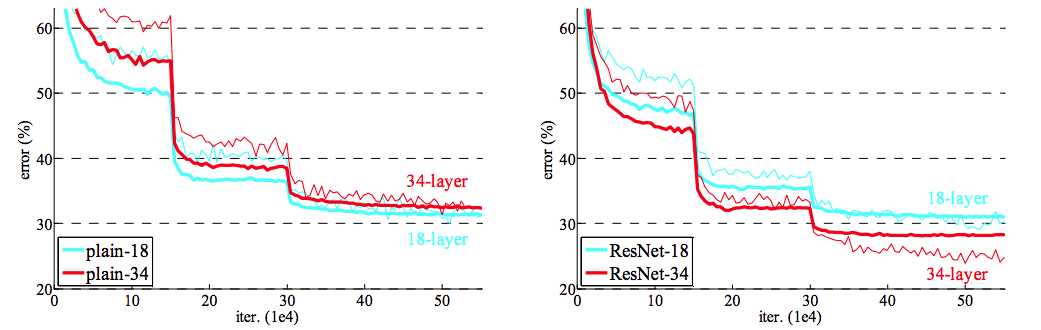
\includegraphics[width = 7in]{../images/annealing}}

\vfill
These Plots are from the original ResNet paper.  Left plot is for CNNs without residual skip connections, the right plot is ResNet.

\vfill
Thin lines are training error, thick lines are validataion error.

\vfill
In all cases $\eta$ is reduced twice, each time by a factor of 2.

\slide{Stationary Distributions}

SGD defines a Markov process in parameter space.

$$\Phi_{i+1} = \Phi_i - \eta \hat{g}_i$$

\vfill
Under Langevin dynamics the stationary distribution of the Markov process must satisfy a certain
differential equation which can be solved.  This gives a general form for
Langevin stationary distributions.

\vfill
In one dimension the stationary distribution is a Boltzman distribution. But this is not generally true in dimension higher than 1.

\slide{Langevin Dynamics With Annealing}

Although the stationary distribution is not a Boltzman distribution, the learning rate $\eta$ acts as a temperature parameter in the sense of the last line below.

\vfill
Let $P_\eta$ be the stationary distribution at learning rate $\eta$.

\begin{eqnarray*}
{\cal L}(\Phi) & = & E_i\;{\cal L}_i(\Phi) \\
\\
{\cal L}(\eta) & = & E_{\Phi \sim P_\eta}\;{\cal L}(\Phi) \\
\\
\lim_{\eta \rightarrow 0} {\cal L}(\eta) & = & {\cal L}(\Phi^*)\;\;\;\mbox{for Langevin dynamics}
\end{eqnarray*}

\slide{A Quadratic Basin Theorem}

\vfill
In practice annealed SGD will converge to a local optimum.

\vfill
We consider stationary distributions restricted to a neighborhood of a (local) optimim $\Phi^*$ satisfying

\begin{eqnarray*}
{\cal L}(\Phi) & = & E_i\;{\cal L}_i(\Phi) \\
\\
{\cal L}_i(\Phi^* + \Delta \Phi) & = & {\cal L}_i + g_i \Delta \Phi + \frac{1}{2} \Delta\Phi^\top H_i \Delta\Phi \\
\\
E_i\; g_i & = & 0\\
\\
E_i\; H_i & & \mbox{is positive definite}
\end{eqnarray*}

\slide{A Quadratic Basin Theorem}

\begin{eqnarray*}
{\cal L}(\Phi) & = & E_i\;{\cal L}_i(\Phi) \\
{\cal L}(\eta) & = & E_{\Phi \sim P_\eta}\;{\cal L}(\Phi) \\
{\cal L}_i(\Phi^* + \Delta \Phi) & = & {\cal L}_i + g_i \Delta \Phi + \frac{1}{2} \Delta\Phi^\top H_i \Delta\Phi \\
E_i\; g_i & = & 0\\
E_i\; H_i & & \mbox{is positive definite} \\
\end{eqnarray*}

\vfill
Theorem:

$${\cal L}(0) = {\cal L}(\Phi^*)\;\;\;\;\;\;\;\;\;\;\;\;{\color{red} \left.\frac{\partial {\cal L}(\eta)}{\partial \eta}\right|_{\eta = 0} \;\;=\;\; \frac{1}{4}\; E_i\; ||g_i||^2}$$

\slide{Analyzing Stationary Distributions}

$${\cal L}(\eta) \approx {\cal L}(\Phi^*) + \eta \left(E_I ||g_i||^2\right)$$

\vfill
$${\cal L}(\Phi^*) = {\cal L}(\eta) - 2({\cal L}(\eta) - {\cal L}(\eta/2)) = {\cal L}(\eta) - 2{\cal L}(\eta/2)$$

\vfill
\centerline{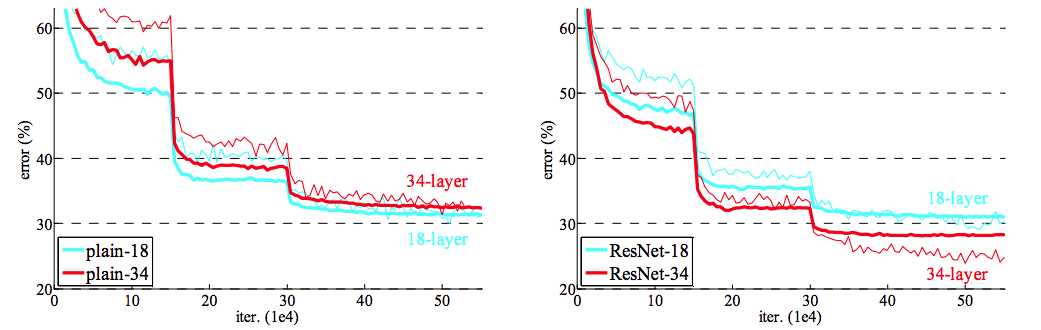
\includegraphics[width = 7in]{../images/annealing}}

\slide{Proof: Observation 1}

\begin{eqnarray*}
{\cal L}(\eta) & = & \;\;\; E_{\Delta \Phi \sim P_\eta}\;E_i \; {\cal L}_i + g_i\Delta _\Phi + \frac{1}{2}\;\Delta \Phi^\top H_i \Delta \Phi \\
\\
& = & E_i\; {\cal L}_i + E_{\Delta \Phi \sim P_\eta} \;(E_i\;g_i) \Delta \Phi + \frac{1}{2}\;\Delta \Phi^\top (E_i\; H_i) \Delta \Phi \\
\\
& = & {\cal L}(\Phi^*)\;\; + \;\; E_{\Delta \Phi \sim P_\eta}\;\;\;\frac{1}{2}\;\Delta \Phi^\top (E_i\;H_i) \Delta \Phi
\end{eqnarray*}

\slide{Proof: Step 1}
Because $P_\eta$ is a stationary distribution we must have

$$E_{\Delta \Phi \sim P_\eta}E_i\; ||\Delta \Phi - \eta (g_i + H_i\Delta \Phi)||^2 = E_{\Delta \Phi \sim P_\eta}\; ||\Delta \Phi||^2$$

\vfill
$$E_{\Delta \Phi \sim P_\eta}E_i\;-2\eta \Delta \Phi^\top (g_i + H_i\Delta \Phi) +\eta^2||(g_i + H_i\Delta \Phi)||^2 = 0$$

\vfill
$$E_{\Delta \Phi \sim P_\eta}\;\left(\frac{1}{2}\Delta \Phi^\top (E_i \;H_i)\Delta \Phi\right) = \frac{\eta}{4}\;E_{\Delta \Phi \sim P_\eta}E_i \;||(g_i + H_i\Delta \Phi)||^2$$

\vfill
$${\color{red} {\cal L}(\eta)  = {\cal L}(\Phi^*) + \frac{\eta}{4}\;E_{\Delta \Phi \sim P_\eta}E_i \;||(g_i + H_i\Delta \Phi)||^2}$$

\slide{Proof Step 2}

\begin{eqnarray*}
{\color{red} {\cal L}(\eta)}  & {\color{red} =} & {\color{red} {\cal L}(\Phi^*) + \frac{\eta}{4}\;E_{\Delta \Phi \sim P_\eta}E_i \;||(g_i + H_i\Delta \Phi)||^2} \\
\\
{\color{red} \left.\frac{\partial {\cal L}(\eta)}{\partial \eta}\right|_{\eta = 0}} & = & \frac{1}{4} \; \lim_{\eta \rightarrow 0} \; E_{\Delta \Phi \sim P_\eta}\; E_i \;||(g_i + H_i\Delta \Phi)||^2 \\
\\
\\
& = & \frac{1}{4} \; E_i\;\lim_{\eta \rightarrow 0}\;E_{\Delta \Phi \sim P_\eta} \;||(g_i + H_i\Delta \Phi)||^2 \\
\\
\\
& {\color{red} =} & {\color{red} \frac{1}{4}\; E_i\;||g_i||^2}
\end{eqnarray*}

\ignore{
\slide{An Original Algorithm Derivation}

\vfill
We will derive a learning rate by maximizing a lower bound on the rate of reduction in training loss.

\vfill
We must consider

\vfill
\begin{itemize}
\item {\bf Gradient Estimation.} The accuracy of $\hat{g}$ as an estimate of $g$.

  \vfill
\item {\bf Gradient Drift (second order structure).} The fact that $g$ changes as the parameters change.
\end{itemize}

\slide{Analysis Plan}

We will calculate a batch size $B^*$ and learning rate $\eta^*$ by optimizing an improvement guarantee for a single batch update.

\vfill
We then use learning rate scaling to derive the learning rate  $\eta_B$ for a batch size $B << B^*$.

\slide{Deriving Learning Rates}

If we can calculate $B^*$ and $\eta^*$ for optimal loss reduction in a single batch
we can calculate $\eta_B$.

\vfill
$$\eta_B = B\;\eta_1$$

\vfill
$$\eta^* = B^* \eta_1$$

\vfill
$$\eta_1 = \frac{\eta^*}{B^*}$$

\vfill
$${\color{red} \eta_B = \frac{B}{B^*} \;\eta^*}$$

\slide{Calculating $B^*$ and $\eta^*$ in One Dimension}

We will first calculate values $B^*$ and $\eta^*$ by optimizing the loss reduction over a single batch update in one dimension.

\vfill
\begin{eqnarray*}
  g & = & \hat{g} \pm \frac{2\hat{\sigma}}{\sqrt{B}} \\
  \\
  \\
  \\
  \hat{\sigma} & = & \sqrt{E_{(x,y) \sim \mathrm{Batch}} \left(\frac{d\;\mathrm{loss}(\beta,x,y)}{d \beta} - \hat{g}\right)^2}
\end{eqnarray*}

\slide{The Second Derivative of $\mathrm{loss}(\beta)$}

\begin{eqnarray*}
  \mathrm{loss}(\beta) & = & E_{(x,y) \sim \mathrm{Train}}\;\mathrm{loss}(\beta,x,y) \\
  \\
  d^2 \mathrm{loss}(\beta)/d \beta^2 & \leq & L \;\;\;\mbox{\Large (Assumption)} \\
  \\
  \mathrm{loss}(\beta - \Delta\beta) & \leq & \mathrm{loss}(\beta) - g\Delta \beta + \frac{1}{2}L\Delta \beta^2 \\
  \\
  \\
  \mathrm{loss}(\beta - \eta\hat{g}) & \leq & \mathrm{loss}(\beta) - g(\eta\hat{g}) + \frac{1}{2}L(\eta\hat{g})^2
\end{eqnarray*}

\slide{A Progress Guarantee}

\begin{eqnarray*}
  \mathrm{loss}(\beta - \eta\hat{g}) & \leq & \mathrm{loss}(\beta) - g(\eta\hat{g}) + \frac{1}{2}L(\eta\hat{g})^2 \\
  \\
  \\
  & = &  \mathrm{loss}(\beta) - \eta (\hat{g} - (\hat{g} -g)) \hat{g} + \frac{1}{2}L\eta^2 \hat{g}^2 \\
  \\
  \\
  & \leq &  \mathrm{loss}(\beta) - \eta \left(\hat{g} - \frac{2\hat{\sigma}}{\sqrt{B}}\right)\hat{g} + \frac{1}{2}L \eta^2 \hat{g}^2
\end{eqnarray*}

\slideplain{Optimizing $B$ and $\eta$}

$$\mathrm{loss}(\beta - \eta\hat{g}) \leq \mathrm{loss}(\beta) - \eta \left(\hat{g} - \frac{2\hat{\sigma}}{\sqrt{B}} \right)\hat{g}  + \frac{1}{2}L \eta^2 \hat{g}^2$$

\vfill
We optimize progress per gradient calculation by optimizing the right hand side divided by $B$.  The derivation at the end of the slides gives

\vfill
$$B^*  =  \frac{16\hat{\sigma}^2}{\hat{g}^2},\;\;\;\;\eta^*  =  \frac{1}{2L}$$

\vfill
$${\color{red} \eta_B} = \frac{B}{B^*} \eta^* = {\color{red} \frac{B \hat{g}^2}{32\hat{\sigma}^2L}}$$

\vfill
Recall this is all just in one dimension.

\slide{Estimating $\hat{g}_{B^*}$ and $\hat{\sigma}_{B^*}$}

$${\color{red} \eta_B = \frac{B \hat{g}^2}{32\hat{\sigma}^2L}}$$

\vfill
We are left with the problem that $\hat{g}$ and $\hat{\sigma}$ are defined in terms of batch size $B^* >> B$.

\vfill
We can estimate $\hat{g}_{B^*}$ and $\hat{\sigma}_{B^*}$ using a running average with a time constant corresponding to $B^*$.

\slide{Estimating $\hat{g}_{B^*}$}

\begin{eqnarray*}
  \hat{g}_{B^*} & = & \frac{1}{B^*} \sum_{(x,y) \sim \mathrm{Batch}(B^*)}\; \frac{d\;\mathrm{Loss}(\beta,x,y)}{d\beta} \\
  \\
  \\
  & = & \frac{1}{N} \sum_{s=t-N+1}^t \hat{g}^s\;\;\;\;\;\mbox{with}\;N= \frac{B^*}{B} \;\mbox{for batch size}\;B \\
  \\
  \\
  \tilde{g}^{t+1} & = & \left(1-\frac{B}{B^*}\right)\tilde{g}^t + \frac{B}{B^*} \hat{g}^{t+1}
\end{eqnarray*}

\vfill
We are still working in just one dimension.

\slide{A Complete Calculation of $\eta$ (in One Dimension)}
\begin{eqnarray*}
  \tilde{g}^{t+1} & = & \left(1-\frac{B}{B^*(t)}\right)\tilde{g}^t + \frac{B}{B^*(t)} \hat{g}^{t+1} \\
  \\
  \tilde{s}^{t+1} & = & \left(1-\frac{B}{B^*(t)}\right)\tilde{s}^t + \frac{B}{B^*(t)} (\hat{g}^{t+1})^2 \\
  \\
  \tilde{\sigma}^t & = & \sqrt{\tilde{s}^t - (\tilde{g}^t)^2} \\
  \\
  B^*(t) &= & \left\{\begin{array}{ll} K & \mbox{for}\;\; t \leq K \\
  16(\tilde{\sigma}^t)^2/((\tilde{g}^t)^2 + \epsilon) & \mbox{otherwise} \end{array}\right.
\end{eqnarray*}

\slide{A Complete Calculation of $\eta$ (in One Dimension)}

$$\eta^t = \left\{\begin{array}{ll} 0 & \mbox{for}\;\;t \leq K \\ \frac{(\tilde{g}^t)^2}{32(\tilde{\sigma}^t)^2L} & \mbox{otherwise}
\end{array}\right.$$

\vfill
As $t \rightarrow \infty$ we expect $\tilde{g}^t \rightarrow 0$ and $\tilde{\sigma}^t \rightarrow \sigma > 0$ which implies
$\eta^t \rightarrow 0$.

\slide{The High Dimensional Case}

So far we have been considering just one dimension.

\vfill
We now propose treating each dimension $\Phi[i]$ of a high dimensional parameter vector $\Phi$ independently using the one dimensional analysis.

\vfill
We can calculate $B^*[i]$ and $\eta^*[i]$ {\bf for each individual parameter} $\Phi[i]$.

\vfill
Of course the actual batch size $B$ will be the same for all parameters.

\slide{A Complete Algorithm}
\begin{eqnarray*}
  \tilde{g}^{t+1}[i] & = & \left(1-\frac{B}{B^*(t)[i]}\right)\tilde{g}^t[i] + \frac{B}{B^*(t)[i]} \hat{g}^{t+1}[i] \\
  \\
  \tilde{s}^{t+1}[i] & = & \left(1-\frac{B}{B^*(t)[i]}\right)\tilde{s}^t[i] + \frac{B}{B^*(t)[i]} \hat{g}^{t+1}[i]^2 \\
  \\
  \tilde{\sigma}^t[i] & = & \sqrt{\tilde{s}^t[i] - \tilde{g}^t[i]^2} \\
  \\
  B^*(t)[i] &= & \left\{\begin{array}{ll} K & \mbox{for}\;\; t \leq K \\
  \lambda_B\tilde{\sigma}^t[i]^2/(\tilde{g}^t[i]^2 + \epsilon) & \mbox{otherwise} \end{array}\right.
\end{eqnarray*}

\slide{A Complete Algorithm}

$$\eta^t[i] = \left\{\begin{array}{ll} 0 & \mbox{for}\;\;t \leq K \\
        \frac{\lambda_\eta\tilde{g}^t[i]^2}{\tilde{\sigma}^t[i]^2} & \mbox{otherwise}
\end{array}\right.$$

\vfill
$$\Phi^{t+1}[i] = \Phi^t[i] - \eta^t[i] \hat{g}^t[i]$$

\vfill
Here we have meta-parameters $K$, $\lambda_B$, $\epsilon$ and $\lambda_\eta$.

\slideplain{Appendix: Optimizing $B$ and $\eta$}

$$\mathrm{loss}(\beta - \eta\hat{g}) \leq \mathrm{loss}(\beta) - \eta \hat{g}\left(\hat{g} - \frac{2\hat{\sigma}}{\sqrt{B}} \right)  + \frac{1}{2}L \eta^2 \hat{g}^2$$

Optimizing $\eta$ we get

\begin{eqnarray*}
 \hat{g}\left(\hat{g} - \frac{2\hat{\sigma}}{\sqrt{B}} \right) & = & L \eta \hat{g}^2
\end{eqnarray*}


\begin{eqnarray*}
\eta^*(B) & = & \frac{1}{L}\left(1 - \frac{2\hat{\sigma}}{\hat{g}\sqrt{B}}\right)
\end{eqnarray*}

\vfill
Inserting this into the guarantee gives
$$\mathrm{loss}(\Phi - \eta \hat{g}) \leq \mathrm{loss}(\Phi) - \frac{L}{2}\eta^*(B)^2\hat{g}^2$$

\slide{Optimizing $B$}

Optimizing progress per sample, or maximizing $\eta^*(B)^2/B$, we get

\begin{eqnarray*}
\frac{\eta^*(B)^2}{B} & = & \frac{1}{L^2}\left(\frac{1}{\sqrt{B}} - \frac{2\hat{\sigma}}{\hat{g}B}\right)^2 \\
\\
0 & = &  - \frac{1}{2} B^{-\frac{3}{2}} + \frac{2\hat{\sigma}}{\hat{g}} B^{-2} \nonumber \\
\\
B^* & = & \frac{16\hat{\sigma}^2}{\hat{g}^2} \\
\\
\eta^*(B^*) = \eta^*  & = & \frac{1}{2L}
\end{eqnarray*}

\ignore{
\slide{Appendix II: A Formal Bound for the Vector Case}

We will prove that minibatch SGD for a {\bf sufficiently large batch size} (for gradient estimation) and a {\bf sufficient small learning rate} (to avoid gradient drift)
is guaranteed (with high probability) to reduce the loss.

\vfill
This guarantee has two main requirements.

\vfill
\begin{itemize}
\item A smoothness condition to limit gradient drift.

  \vfill
\item A bound on the gradient norm allowing high confidence gradient estimation.
\end{itemize}
  

\slide{Smoothness: The Hessian}

We can make a second order approximation to the loss.

\begin{eqnarray*}
  \ell(\Phi + \Delta \Phi) & \approx & \ell(\Phi) + g^\top \Delta \Phi + \frac{1}{2} \Delta \Phi^\top H \Delta \Phi \\
  \\
  g & = & \nabla_\Phi\;\ell(\Phi) \\
  \\
  H & = & \nabla_\Phi \nabla_\Phi\; \ell(\Phi)
\end{eqnarray*}


\slide{The Smoothness Condition}

We will assume

$$||H\Delta \Phi|| \leq L||\Delta \Phi||$$

We now have

\vfill
$$\Delta \Phi^\top H \Delta \Phi \leq L ||\Delta \Phi||^2$$

\vfill
Using the second order mean value theorem one can prove

\begin{eqnarray*}
  \ell(\Phi + \Delta \Phi)  & \leq &    \ell(\Phi) + g^\top \Delta \Phi + \frac{1}{2} L ||\Delta \Phi||^2
\end{eqnarray*}


\slide{A Concentration Inequality for Gradient Estimation}

Consider a vector mean estimator where the vectors $g_n$ are drawn IID.

$$g_n = \nabla_\Phi \ell_n(\Phi) \;\;\;\;\;\;\hat{g} = \frac{1}{k} \sum_{n=1}^k g_n \;\;\;\; \;\;\;\;\;\;\;\; g = \expectsub{n}{\nabla_\Phi\;\ell_n(\Phi)}$$

\vfill
{\bf If with probability 1 over the draw of $n$ we have $|(g_n)_i - g_i| \leq b$ for all $i$} then with probability of at least $1-\delta$ over the draw of the sample

\vfill

$$||\hat{g} - g|| \leq \frac{\eta}{\sqrt{k}} \;\;\;\;\;\;\;\;\;\;\;\;\;\; \eta = b\left(1 + \sqrt{2 \ln (1/ \delta) }\right)$$


\vfill
{\huge Norkin and Wets ``Law of Small Numbers as Concentration Inequalities ...'', 2012, theorem 3.1}

\begin{eqnarray*}
 \ell(\Phi + \Delta \Phi) & \leq &   \ell(\Phi) + g^\top \Delta \Phi + \frac{1}{2} L ||\Delta \Phi||^2 \\
  \\
\ell(\Phi - \eta\widehat{g}) & \leq & \ell(\Phi) - \eta g^\top \widehat{g} + \frac{1}{2}L \eta^2 ||\widehat{g}||^2\\
  \\
  & = &  \ell(\Phi) - \eta (\widehat{g} - (\widehat{g} -g))^\top \widehat{g} + \frac{1}{2}L\eta^2 ||\widehat{g}||^2 \\
  \\
  & = &  \ell(\Phi) - \eta ||\widehat{g}||^2 + \eta(\widehat{g} -g)^\top \widehat{g} + \frac{1}{2}L \eta^2 ||\widehat{g}||^2 \\
  \\
  & \leq &  \ell(\Phi) - \eta ||\widehat{g}||^2 + \eta\frac{\eta}{\sqrt{k}}||\widehat{g}|| + \frac{1}{2}L \eta^2 ||\widehat{g}||^2 \\
  \\
  & = & \ell(\Phi) - \eta ||\widehat{g}||\left(||\widehat{g}|| - \frac{\eta}{\sqrt{k}} \right)  + \frac{1}{2}L \eta^2 ||\widehat{g}||^2 \\
\end{eqnarray*}

\slideplain{Optimizing $\eta$}

Optimizing $\eta$ we get

\begin{eqnarray*}
 ||\widehat{g}||\left(||\widehat{g}|| - \frac{\eta}{\sqrt{k}} \right) & = & - L \eta ||\widehat{g}||^2
\end{eqnarray*}


\begin{eqnarray*}
\eta & = & \frac{1}{L}\left(1 - \frac{\eta}{||\widehat{g}||\sqrt{k}}\right)
\end{eqnarray*}

\vfill
Inserting this into the guarantee gives
$$\ell(\Phi - \eta \widehat{g}) \leq \ell(\Phi) - \frac{L}{2}\eta^2||\widehat{g}||^2$$

\slide{Optimizing $k$}

Optimizing progress per sample, or maximizing $\eta^2/k$, we get.

\begin{eqnarray*}
\frac{\eta^2}{k} & = & \frac{1}{L^2}\left(\frac{1}{\sqrt{k}} - \frac{2\hat{\sigma}}{||\widehat{g}||k}\right)^2 \\
\\
0 & = &  - \frac{1}{2} k^{-\frac{3}{2}} + \frac{2\hat{\sigma}}{||\widehat{g}||} k^{-2} \nonumber \\
\\
k & = & \left(\frac{22\hat{\sigma}}{||\widehat{g}||}\right)^2 \\
\\
\eta & = & \frac{1}{2L}
\end{eqnarray*}
}

}

\slide{END}

} \end{document}

